\documentclass[times, utf8, zavrsni, numeric]{fer}
\setlength{\parindent}{0em}
\tolerance=1
\emergencystretch=\maxdimen
\hyphenpenalty=10000
\hbadness=10000
\graphicspath{{../Slike/}}
\usepackage{hyperref}
\hypersetup{
	colorlinks=true,
	citecolor=black,
	linkcolor=black,
	urlcolor=cyan,
	pdflinkmargin=5pt
}

\begin{document}

% TODO: Navedite broj rada.
\thesisnumber{000}

\title{POVEZIVANJE VIRTUALNOG I STVARNOG OSVJETLJENJA KORIŠTENJEM UNREAL SUSTAVA}

\author{Bernard Bačani}

\maketitle

% Ispis stranice s napomenom o umetanju izvornika rada. Uklonite naredbu \izvornik ako želite izbaciti tu stranicu.
\izvornik

% Dodavanje zahvale ili prazne stranice. Ako ne želite dodati zahvalu, naredbu ostavite radi prazne stranice.
\zahvala{Zahvaljujem se Tiboru Jakovecu što je svaki dan išao sa mnom u menzu i svaki dan kasnio.}

\tableofcontents

\chapter{Uvod}
Uvod rada. Nakon uvoda dolaze poglavlja u kojima se obrađuje tema.

\chapter{Virtualna produkcija}
Filmska produkcija je izuzetno kompleksan proces koji je tipično linearan te se sastoji od razvoja, pretprodukcije, produkcije i postprodukcije (slika \ref{fig:slika 2-1}). Problem tradicionalne produkcije je izoliranost sudionika u pojedinoj fazi i neprilagodljivost promjenama na samom setu. Konačna verzija scene ne zna se do samog kraja produkcije, što uvelike otežava cijeli proces snimanja.\newline

\begin{figure}[htp]
	\centering
	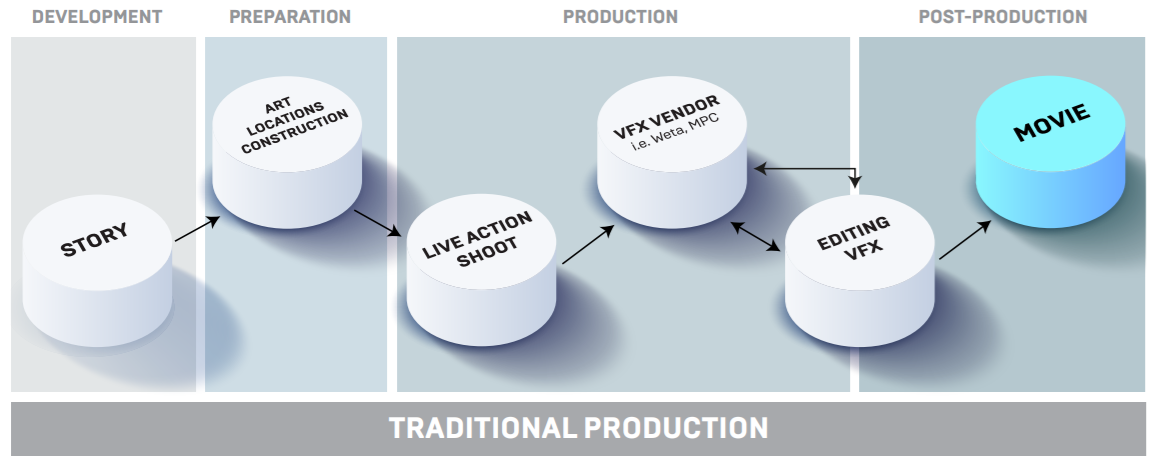
\includegraphics[width=\linewidth]{slika 2-1.png}
	\caption{Tradicionalna produkcija \cite{vpguide1}}
	\label{fig:slika 2-1}
\end{figure}

Virtualna produkcija je metoda slična agilnom razvoju, gdje se korištenjem pogonskog sklopa igara (engl. \emph{game engine}) prati kretnja kamere u stvarnom vremenu te se pozadinski sadržaj prikazuje na LED ekranu. Za razliku od tradicionalne, virtualna produkcija uvodi fleksibilnost u snimanje, omogućujući promjenu priče ili bilo kojeg dijela seta uz prisutnost cijelog tima, čime se štedi na vremenu i resursima (slika \ref{fig:slika 2-2}).

\pagebreak

\begin{figure}[htp]
	\centering
	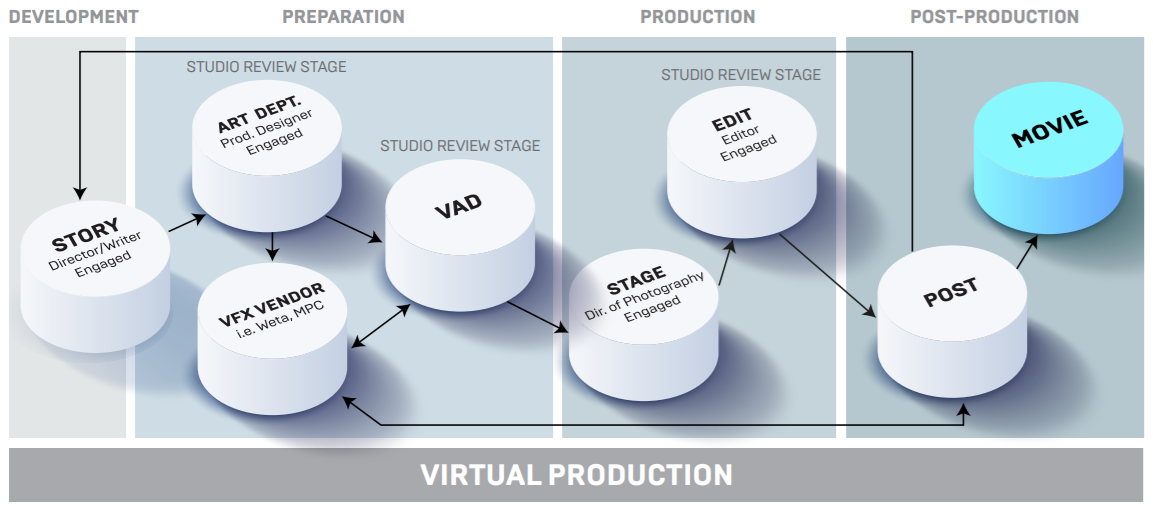
\includegraphics[width=\linewidth]{slika 2-2.png}
	\caption{Virtualna produkcija \cite{vpguide1}}
	\label{fig:slika 2-2}
\end{figure}

\section{Slučajevi upotrebe}
Vizualizacija je vjerojatno najčešći oblik upotrebe virtualne produkcije, a posebice predvizualizacija, koja u novoj paradigmi pruža prvi uvid u ideje i sredstva koja će se koristiti kroz produkciju \cite{vpguide2}. Poznata uporaba ove tehnike je u seriji \emph{The Mandalorian} (2019.-) gdje je virtualna produkcija bila korištena u snimanju više od pola cijele prve sezone (slika \ref{fig:slika 2-3}).\newline

Osim u filmovima i serijama može se koristiti u predvizualizaciji raznih javnih događaja poput koncerata. Primjerice, tvrtka Moment Factory je u 2021. godini objavila projekt \emph{DMX Previs}, digitalni svjetlosni šou (engl. \emph{light show}) napravljen koristeći DMX plugin u Unrealu (slika \ref{fig:slika 2-4}) koji je sličan primjeru iz stvarnog života te ga se može i upravljati upravljačkom konzolom za osvjetljenje.\newline

Također, virtualna produkcija koristi se za hvatanje pokreta (engl. \emph{motion capture}) - praćenja pokreta objekata ili glumaca za animaciju digitalnih modela i kod vizualnih efekata u kameri (engl. \emph{in-camera visual effects}, skraćeno in-camera VFX).

\begin{figure}[htp]
	\centering
	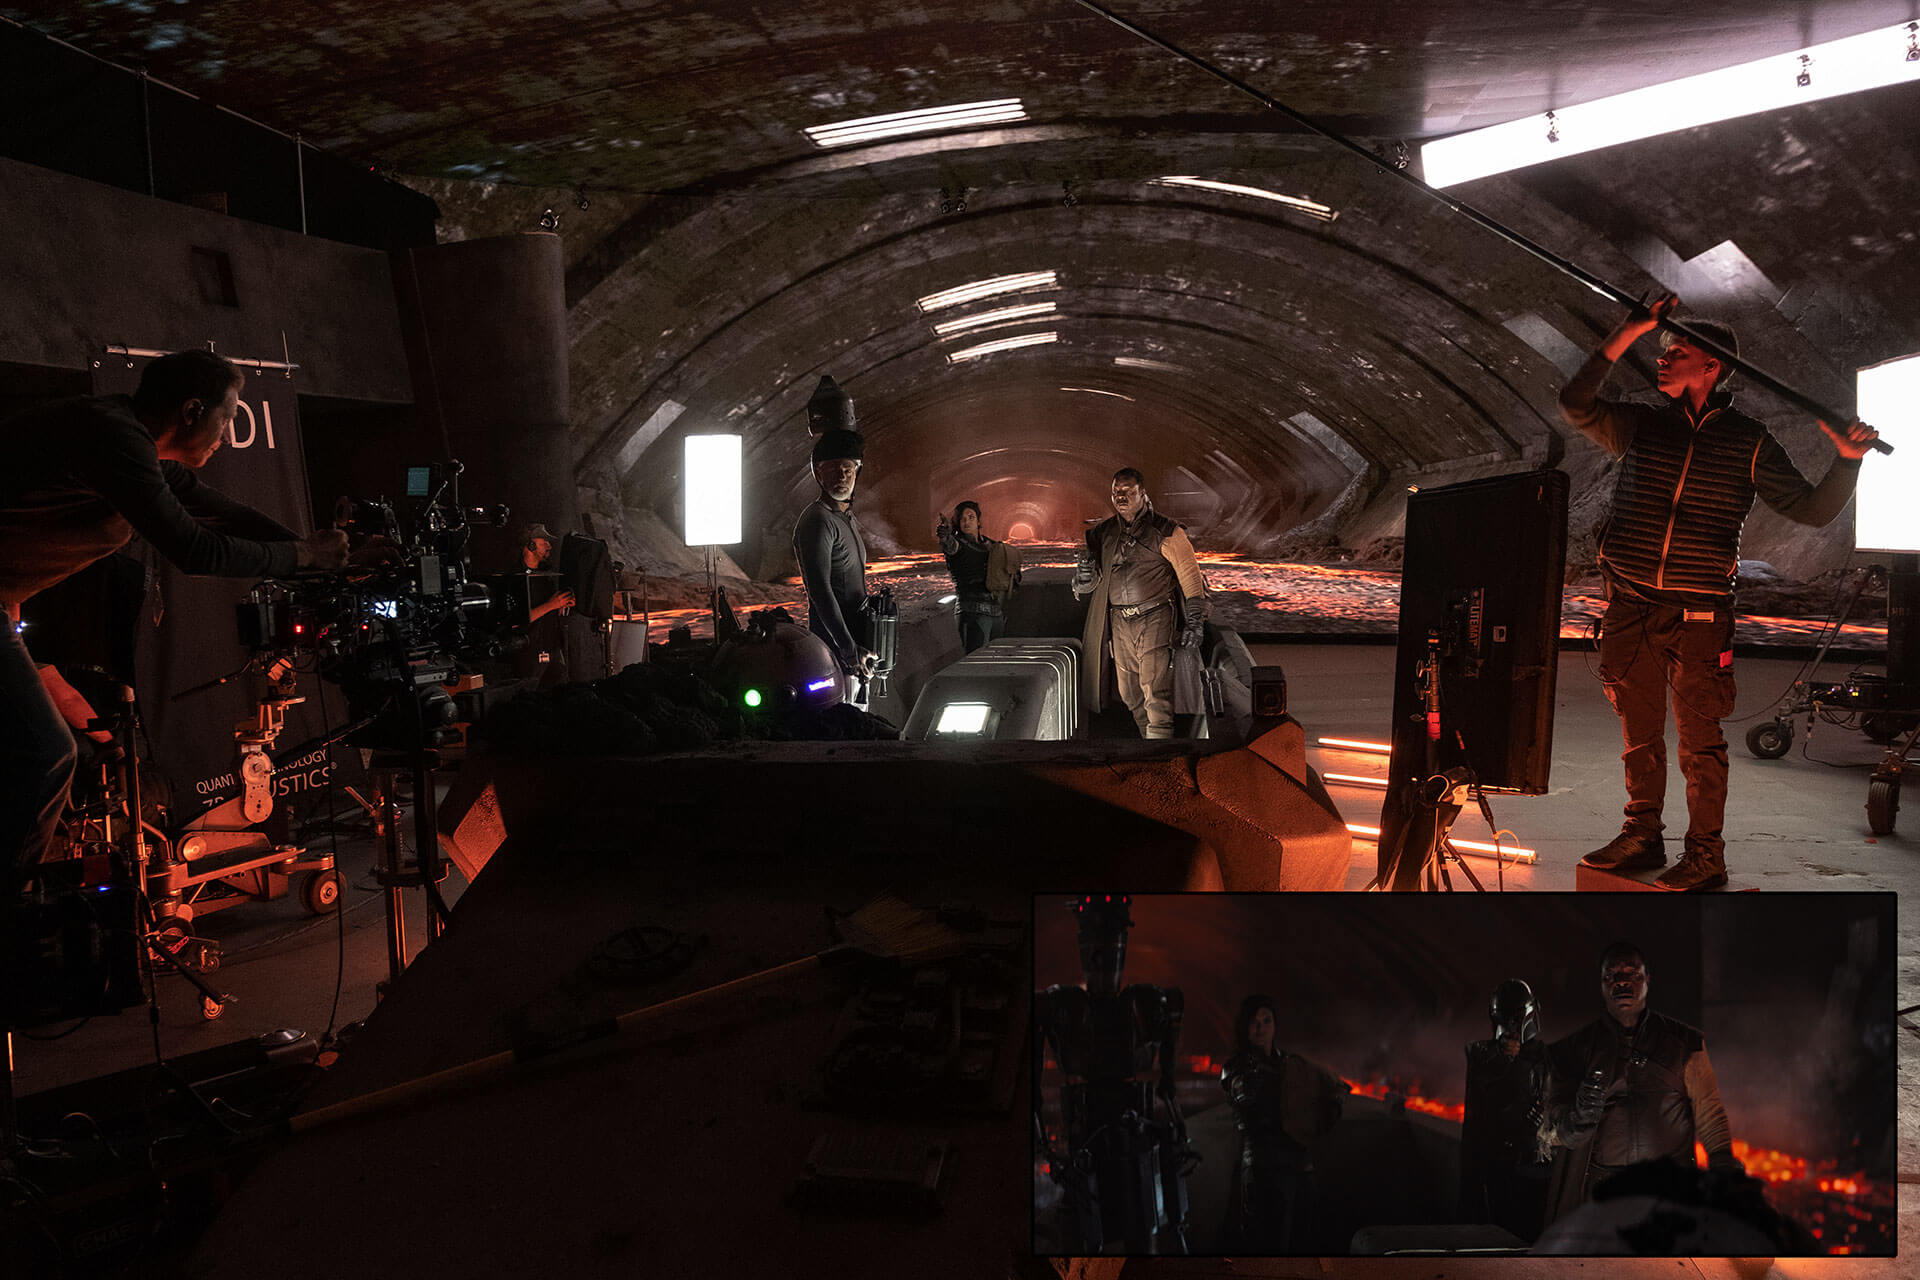
\includegraphics[width=\linewidth]{slika 2-3.png}
	\caption{Set u seriji \emph{The Mandalorian} \cite{mandalorian}}
	\label{fig:slika 2-3}
\end{figure}

\begin{figure}[htp]
	\centering
	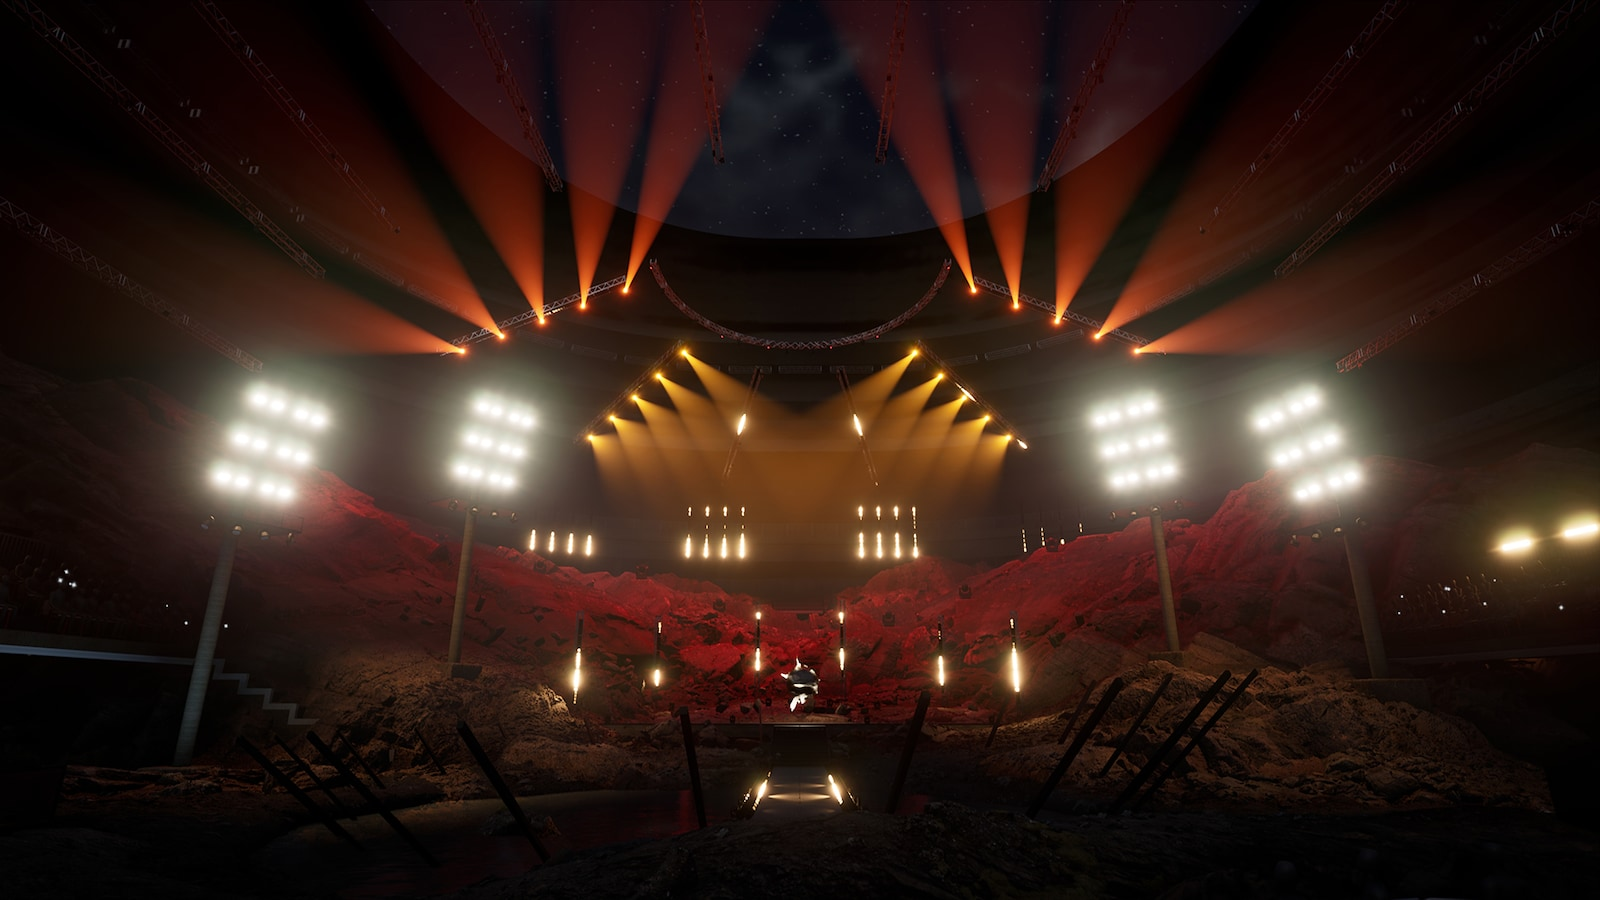
\includegraphics[width=\linewidth]{slika 2-4.png}
	\caption{Svjetlosni šou \emph{DMX Previs} \cite{dmx_previs}}
	\label{fig:slika 2-4}
\end{figure}

\pagebreak

\section{Opis prototipa}

\chapter{Upravljanje osvjetljenjem}

\section{DMX}

\subsection{Kontroleri}

\subsection{Rasvjetna tijela}

\subsection{Signalna komunikacija}

\section{Mrežni protokoli za prijenos podataka}

\subsection{Art-Net}

\subsection{sACN}

\chapter{Model rješenja}
Upravljačka konzola za osvjetljenje je uređaj kojim se upravlja svjetlosnim i drugim uređajima putem upravljačkog protokola. Zbog povećane količine uređaja na pozornici, osim komuniciranja direktno ili preko USB-a, neke konzole također mogu komunicirati putem mreže kako bi se olakšala kontrola nad složenim sustavima. Za ovaj rad korišten je simulator konzole koji šalje podatke preko ethernet protokola.\newline

Svjetlosni efekti korišteni u simulaciji su nalik na one u javnima događajima, poput koncerata gdje se koriste primjerice reflektori, laseri, dimni efekti i drugo.
Zatim, simulacija se integrira s postojećim sustavom za detekciju položaja kamere u kojem se pomoću stvarne kamere upravlja virtualnom kamerom u stvarnom vremenu.

\section{Simulacija osvjetljenja}
Simulacija je zamišljena kao predvizualizacija mini pozornice u kazalištu. Pozornica sadrži nekoliko reflektora, statičnih svjetala i lasera. Svjetlosnim uređajima se upravlja simulatorom konzole te se svjetla pale i gase, mijenja im se pozicija, pojačava ili smanjuje intenzitet i slično. Promatra se unaprijed programiran skup naredbi, a zatim slanje naredbi u stvarnom vremenu i njihovo kašnjenje. Simulacija je uspješna ako je dobiven rezultat sličan korištenju prave konzole te je utjecaj kašnjenja minimalan.

\pagebreak

\section{Integracija s prototipom}
Povezivanje s prototipom ostvaruje se korištenjem stvarne kamere, \emph{HTC Vive Trackera}, \emph{Base Stationa} i LED zaslona. Kako se simulacija izvodi, kretanjem stvarne kamere mapiraju se pokreti u virtualnu kameru te se time krećemo po pozornici. Ispred LED zaslona stavljaju se objekti u stvarnom životu te se snima smješten objekt u virtualnoj scenu. Integracija je uspješna ako dobijemo dojam da se objekt stvarno nalazi na pozornici, a simulirana svjetlost nalikuje stvarnoj svjetlosti.

\chapter{Zaključak}
Zaključak.

\raggedright
\bibliography{literatura}
\bibliographystyle{fer}

\begin{sazetak}
Sažetak na hrvatskom jeziku.

\kljucnerijeci{Ključne riječi, odvojene zarezima.}
\end{sazetak}

\engtitle{CONNECTING VIRTUAL AND REAL LIGHTING USING THE UNREAL SYSTEM}
\begin{abstract}
Abstract.

\keywords{Keywords.}
\end{abstract}

\end{document}
